% !TEX TS-program = pdflatexmk
\documentclass{./packages/optica-article}

\graphicspath{{images/}{practica2/images}}

\journal{opticajournal}


\usepackage{csvsimple}
\usepackage{siunitx}
\usepackage{graphicx}
\usepackage{physics}
\usepackage{booktabs}
\usepackage{tikz}
\usetikzlibrary{positioning}

\tikzset{>=stealth}

% cref instead of ref
\usepackage{cleveref}

\newcommand{\sinc}{\textrm{sinc}}
\newcommand\conv{\circledast}


% Set the article type
\articletype{Research Article}

% \usepackage{lineno}
% \linenumbers

\begin{document}

\title{El efecto Talbot}

\author{Adriana Mamani Lazarte\authormark{1} Alex G. Recuenco\authormark{1}, and Carlos España Castaño\authormark{1}}

\address{\authormark{1}Universidad Complutense de Madrid, Madrid, PC 28040, España}

\section{Introducción}
En la práctica realizada primeramente se aprendió a realizar montajes experimentales de sistemas ópticos, de tal manera que el mismo este alineado de manera correcta y el haz se encuentre colimado. Se estudia experimentalmente el efecto de Talbot que es la reproducción de campos periódicos durante la propagación en el espacio
libre en el régimen de Fresnel para ciertas distancias. Por otra parte, se construyó un sistema para la observación y medida del espectro de Fourier de un objeto 2D (en este caso una lámina fotográfica). Se analiza la difracción de la iluminación coherente de una imagen al mover la cámara con respecto a la imagen.

\section{Desarrollo}

\subsection{Marco Práctico}
    \begin{enumerate}
    \item Observación efecto de Talbot
Se trabaja con el siguiente esquema:

    \begin{figure}[h]
    \centering
    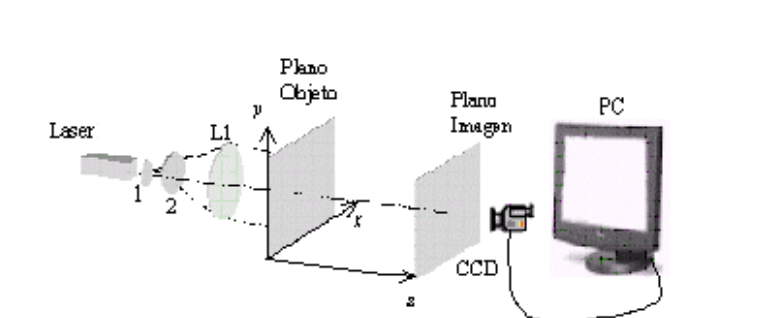
\includegraphics[scale=1]{/sistematalbot.png}
    \caption{ Esquema del banco óptico, (1) filtro espacial, (2) atenuador, L1 lente colimadora, cámara CCD y PC para efectuar el registro.}
    \label{talbot}
    \end{figure}
    
    
Se observó la evolución del campo difractado al alejar la cámara CCD del plano del objeto, y se apuntó las distancias descritas a continuación:\par


Se registraron las imágenes y las distancias donde se observaron:\par
    \begin{figure}[h]
    \centering
    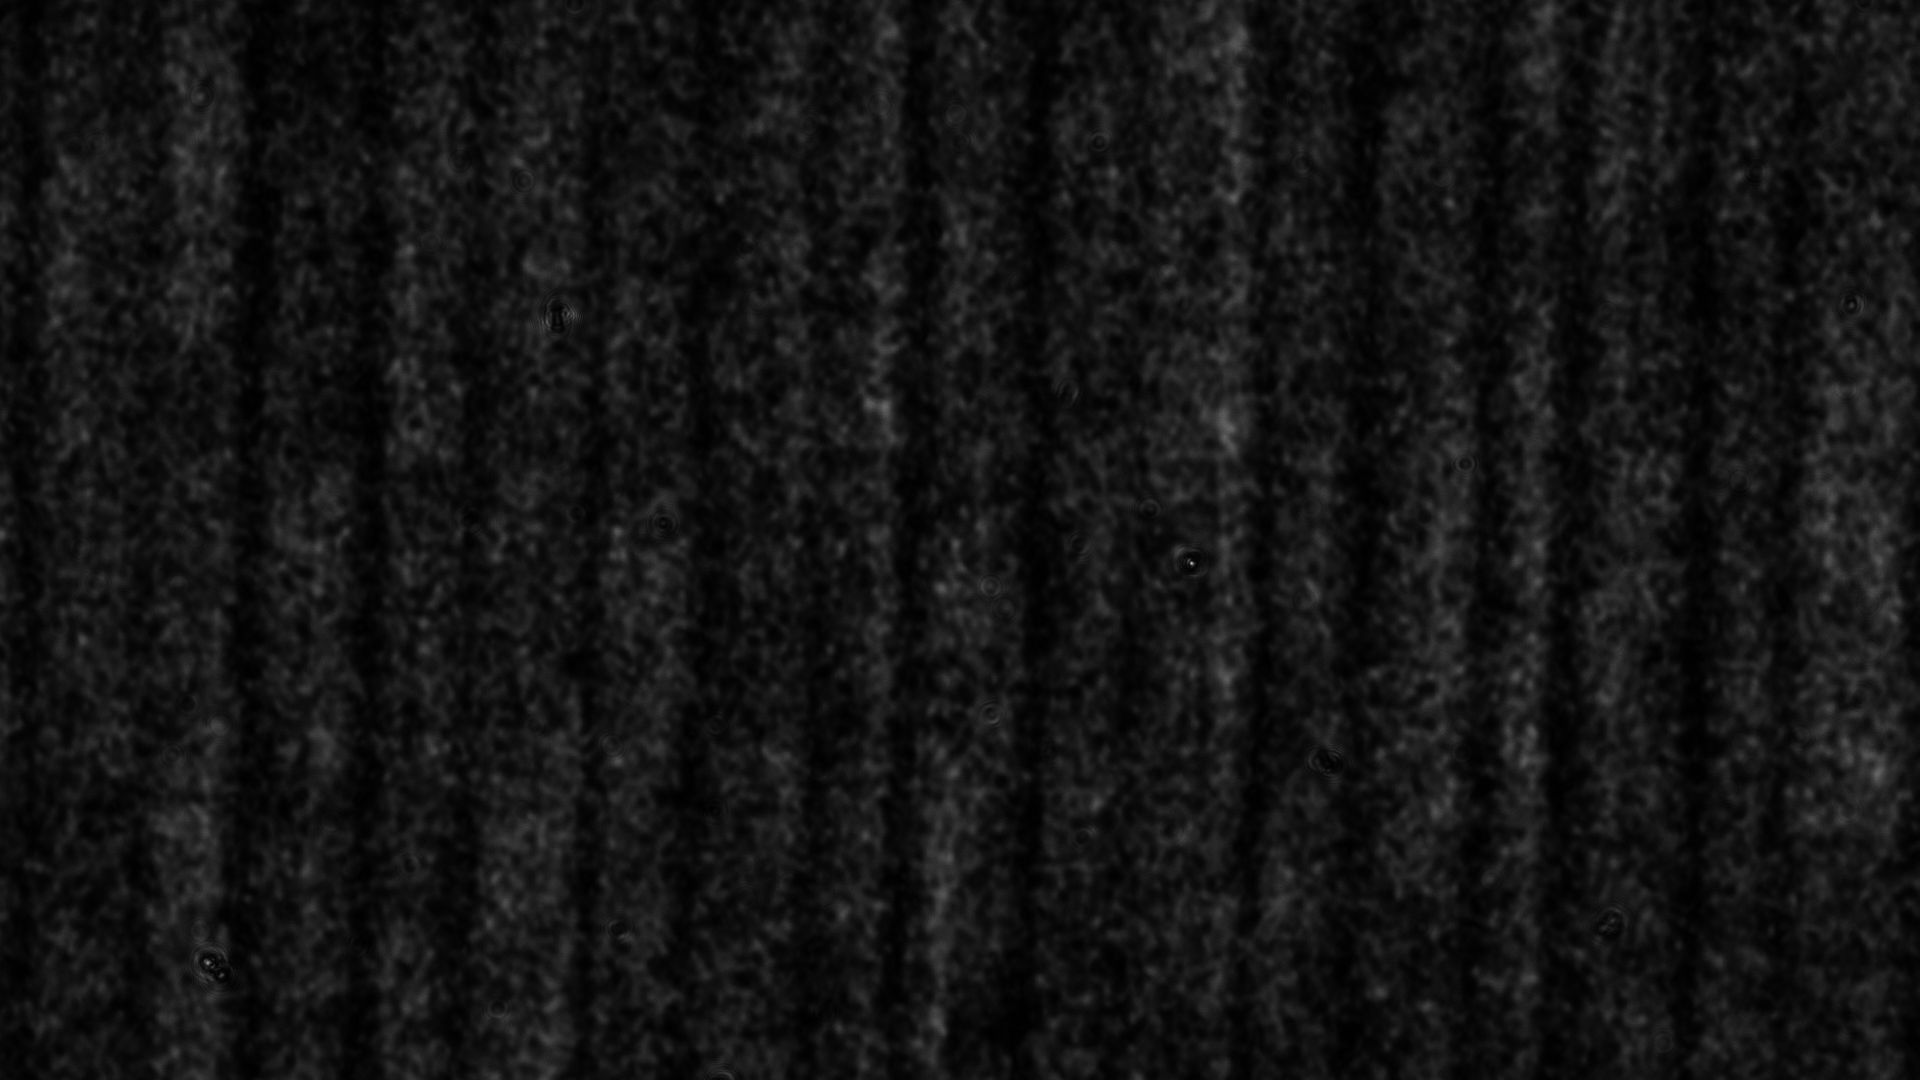
\includegraphics[scale=0.2]{/parte2-talbot/4.9cm-talbot7.png}
    \caption{ Talbot a distancia 1}
    \label{talbot1}
    \end{figure}
    
    \begin{figure}[h]
    \centering
    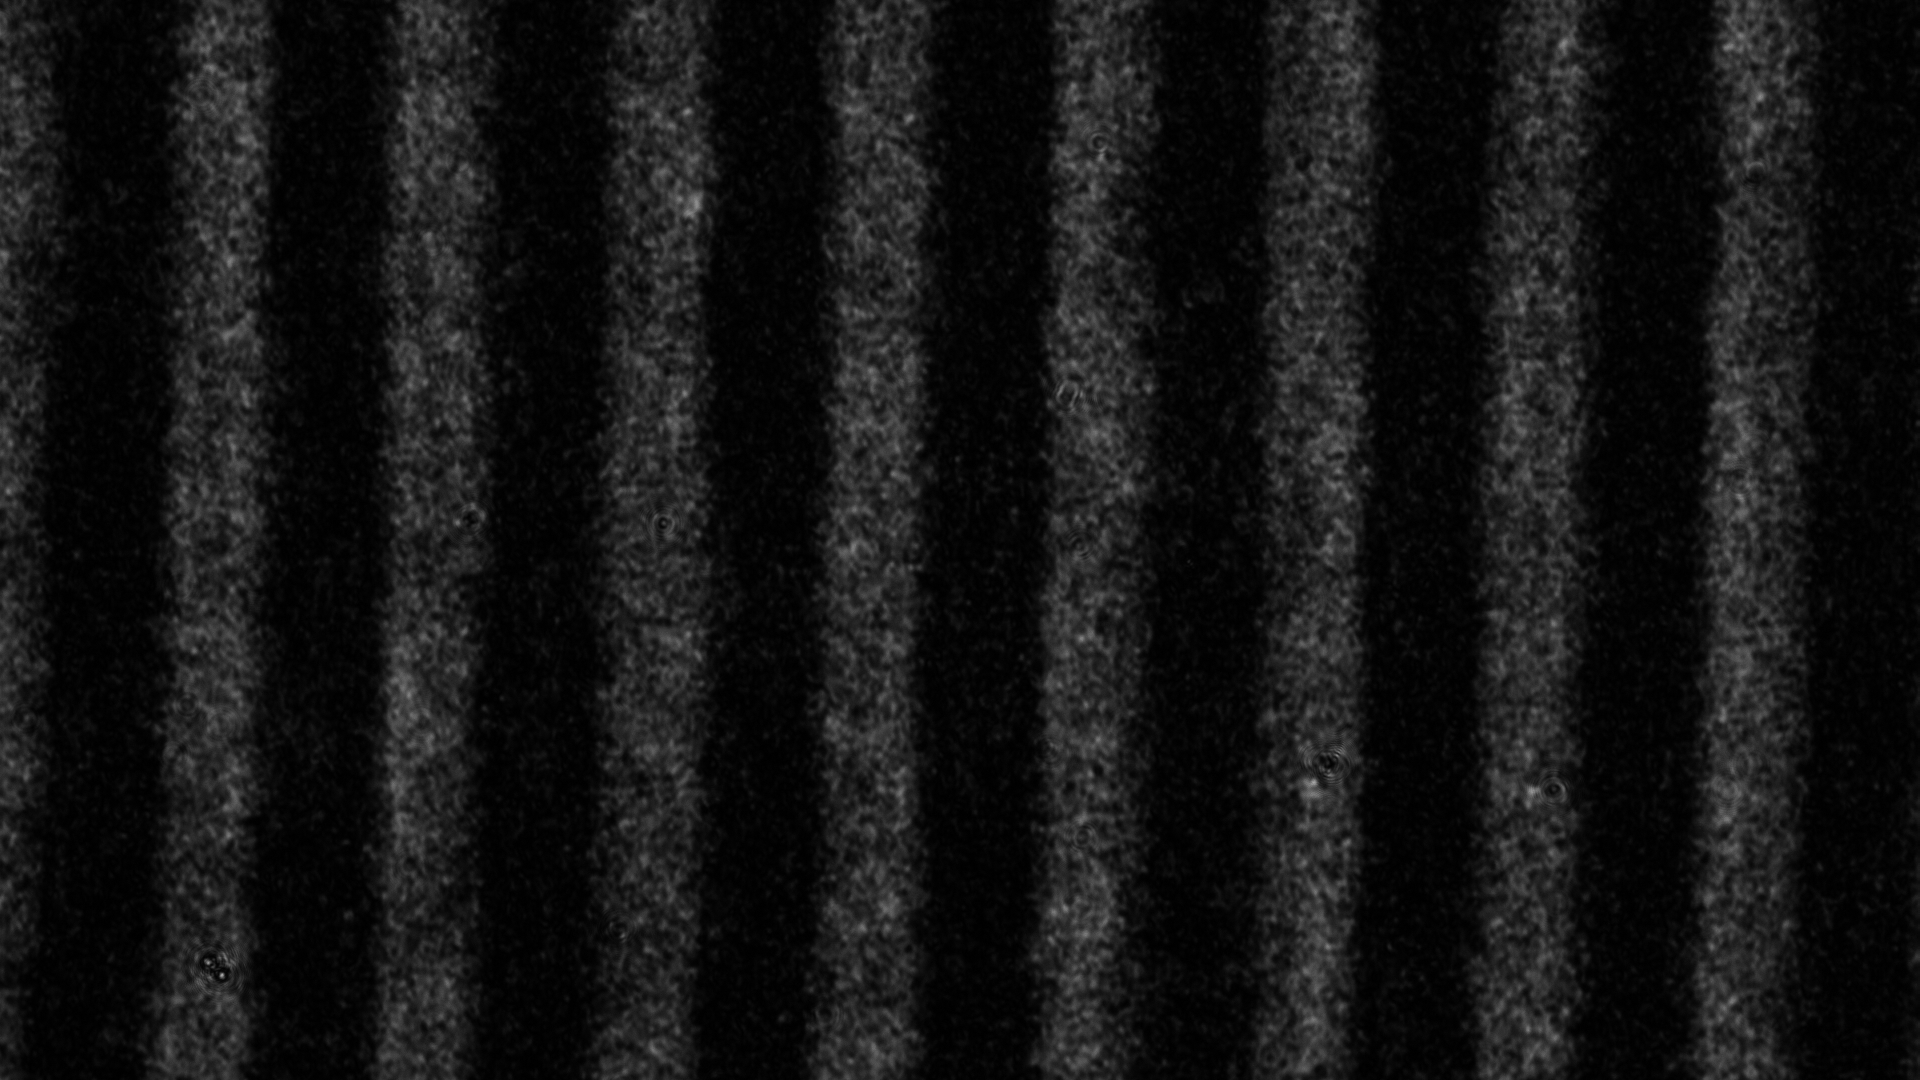
\includegraphics[scale=0.15]{/parte2-talbot/23.9-talbot.png}
    \caption{ Talbot a distancia 2}
    \label{talbot2}
    \end{figure}
    
    \begin{figure}[h]
    \centering
    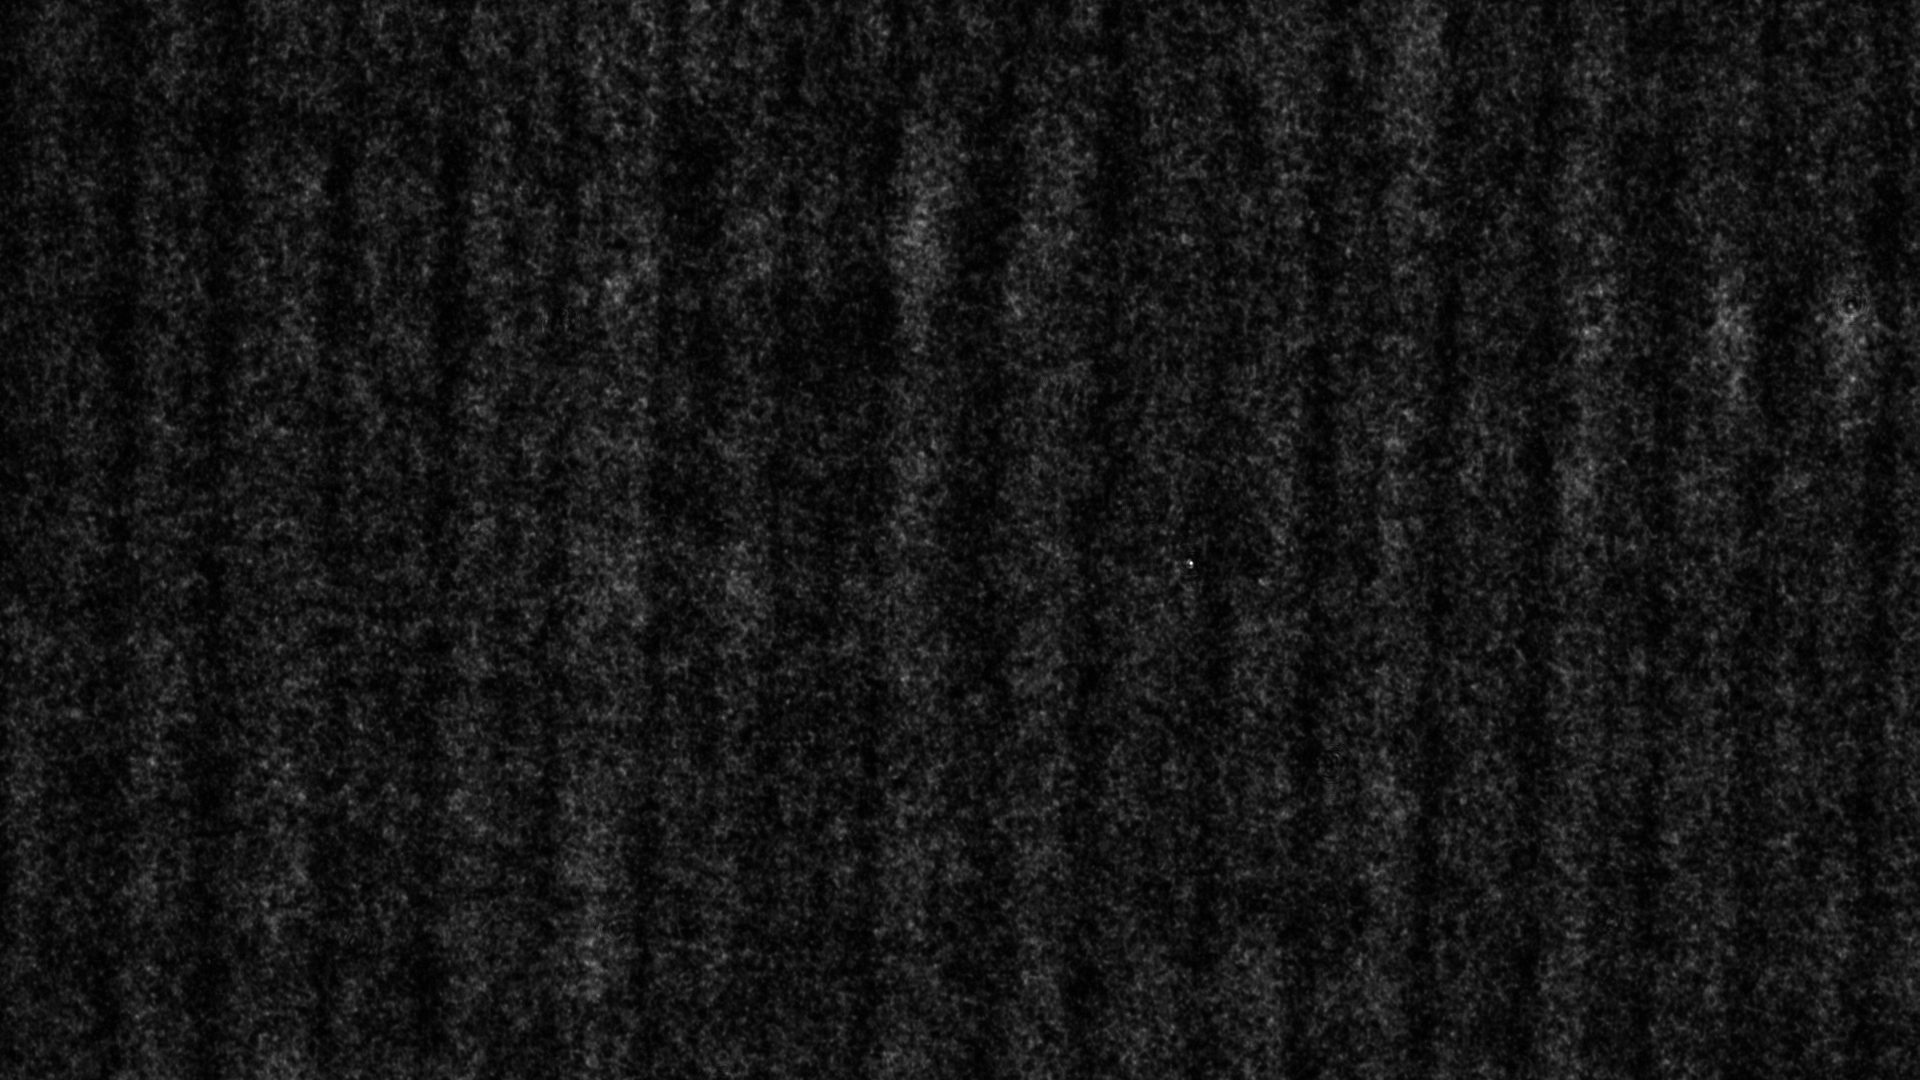
\includegraphics[scale=0.15]{/parte2-talbot/42.2-talbot.png}
    \caption{ Talbot a distancia 3}
    \label{talbot3}
    \end{figure}
    
    \begin{figure}[h]
    \centering
    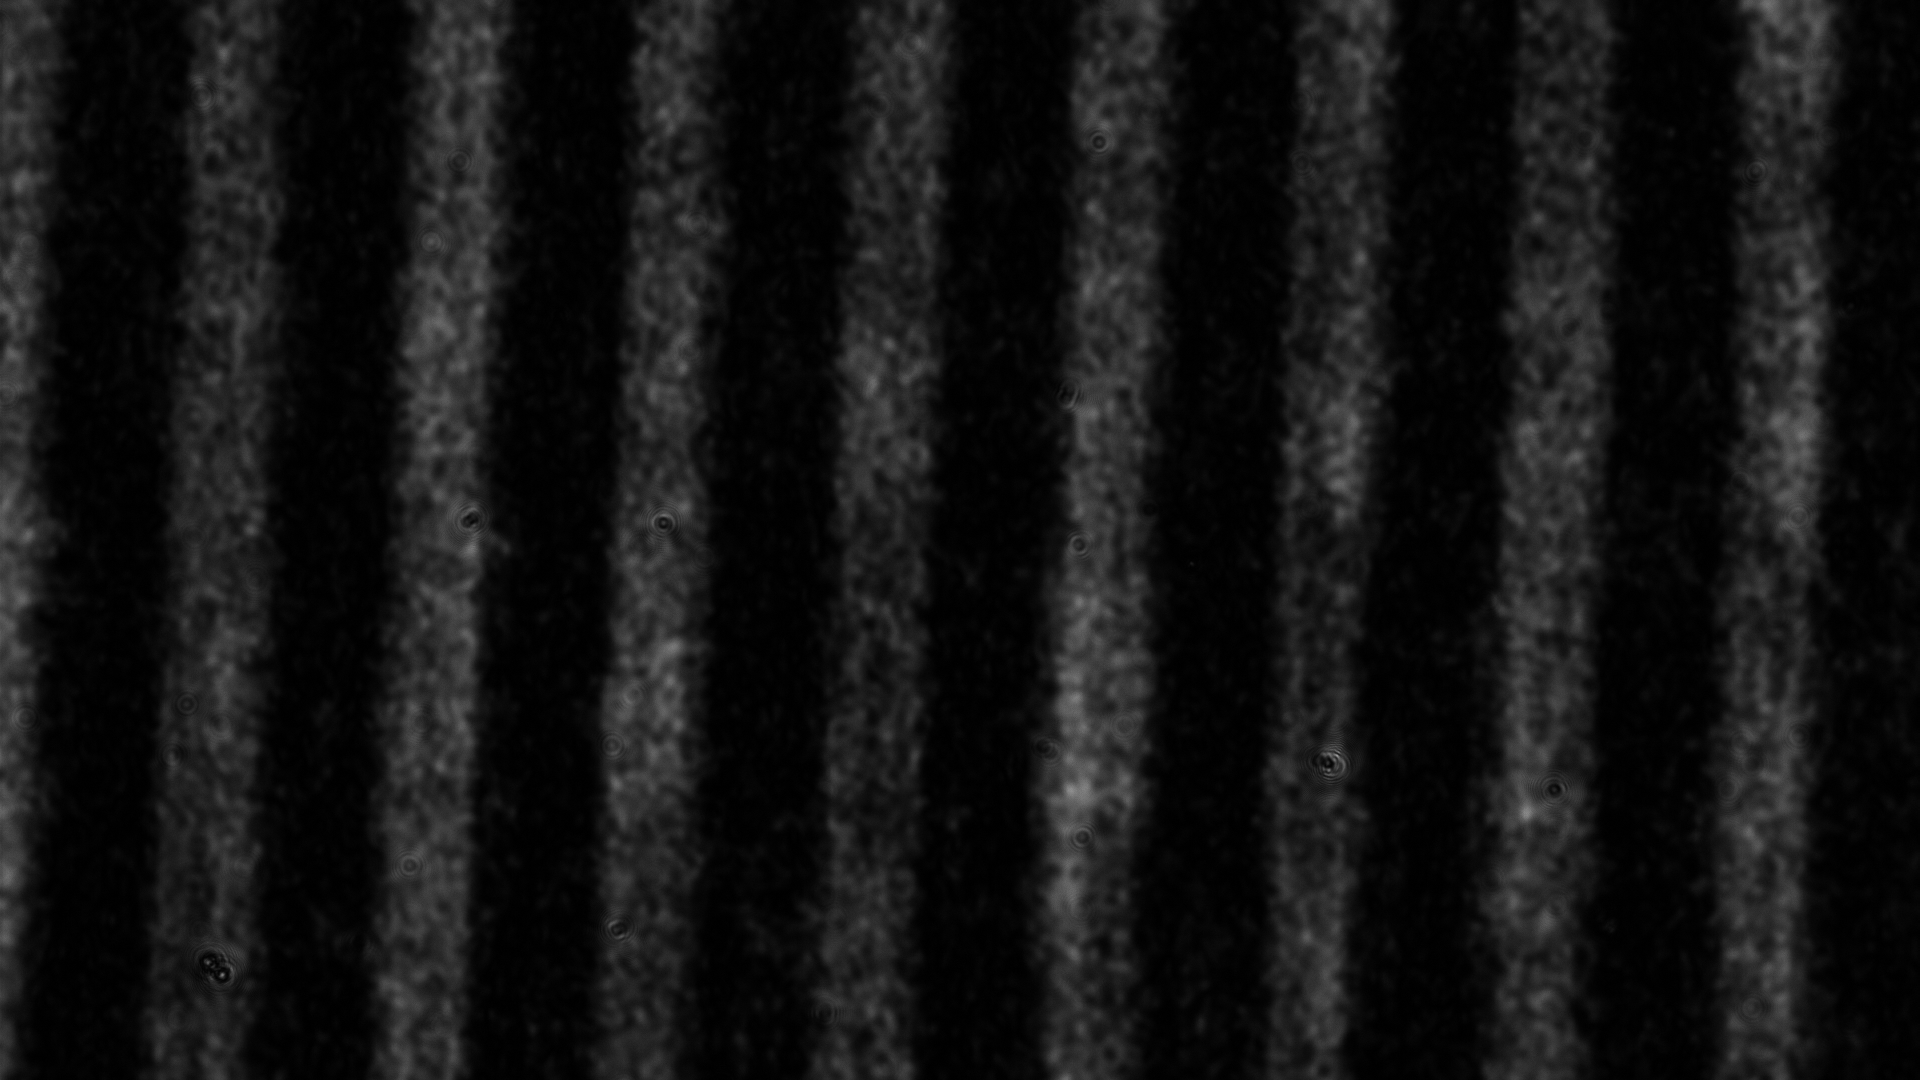
\includegraphics[scale=0.15]{/parte2-talbot/54.8-2a-talbot.png}
    \caption{ Talbot a distancia 3}
    \label{talbot3}
    \end{figure}
    

Se estima la distancia de talbot siendo:
\par

y el periodo de la red: \par


Se registró las imágenes mostradas a continuacion:

¿Las imágenes siempre son periódicas?



    \item Espectro de Fourier
Se realiza la experimentación bajo el diseño del siguiente montaje:

\begin{figure}[h]
    \centering
    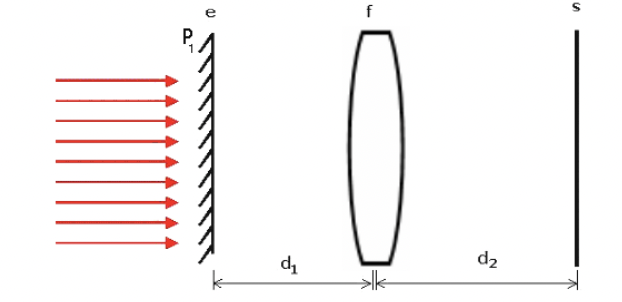
\includegraphics[scale=1]{sistemaespectrodefourier.png}
    \caption{Esquema del montaje experimental para la observación del espectro de Fourier de un objeto plano. }
    \label{fouriersistema}
    \end{figure}

En el sistema armado se utilizaron lentes focales diferentes, un polarizador como atenuador y un diafragma para disminuir la influencia de luz parasita.

Se observaron los espectros de Fourier en los siguientes escenarios: \par


\begin{figure}[h]
    \centering
    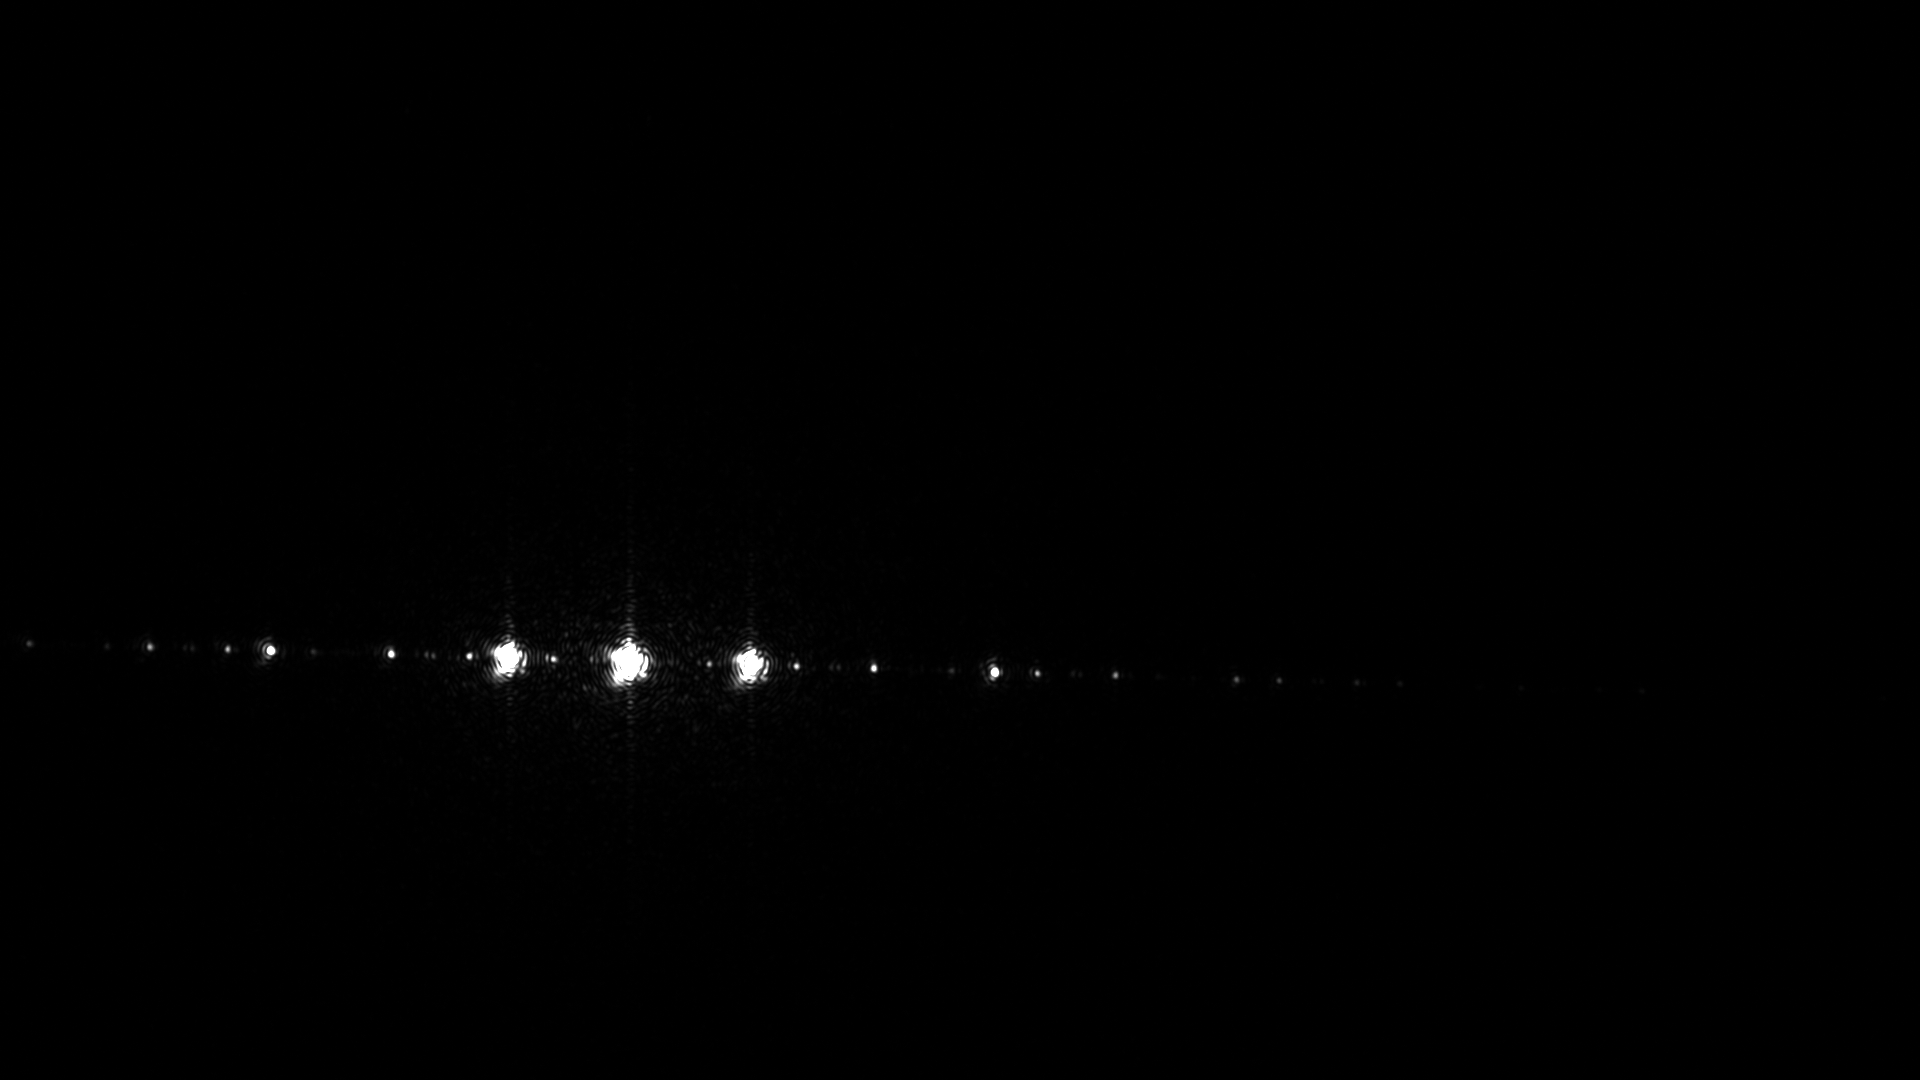
\includegraphics[scale=0.15]{/parte3-fourier/fourier_transform_-20-lense-20-camera.png}
    \caption{Esquema del montaje experimental para la observación del espectro de Fourier de un objeto plano. }
    \label{fourier1}
    \end{figure}

\begin{figure}[h]
    \centering
    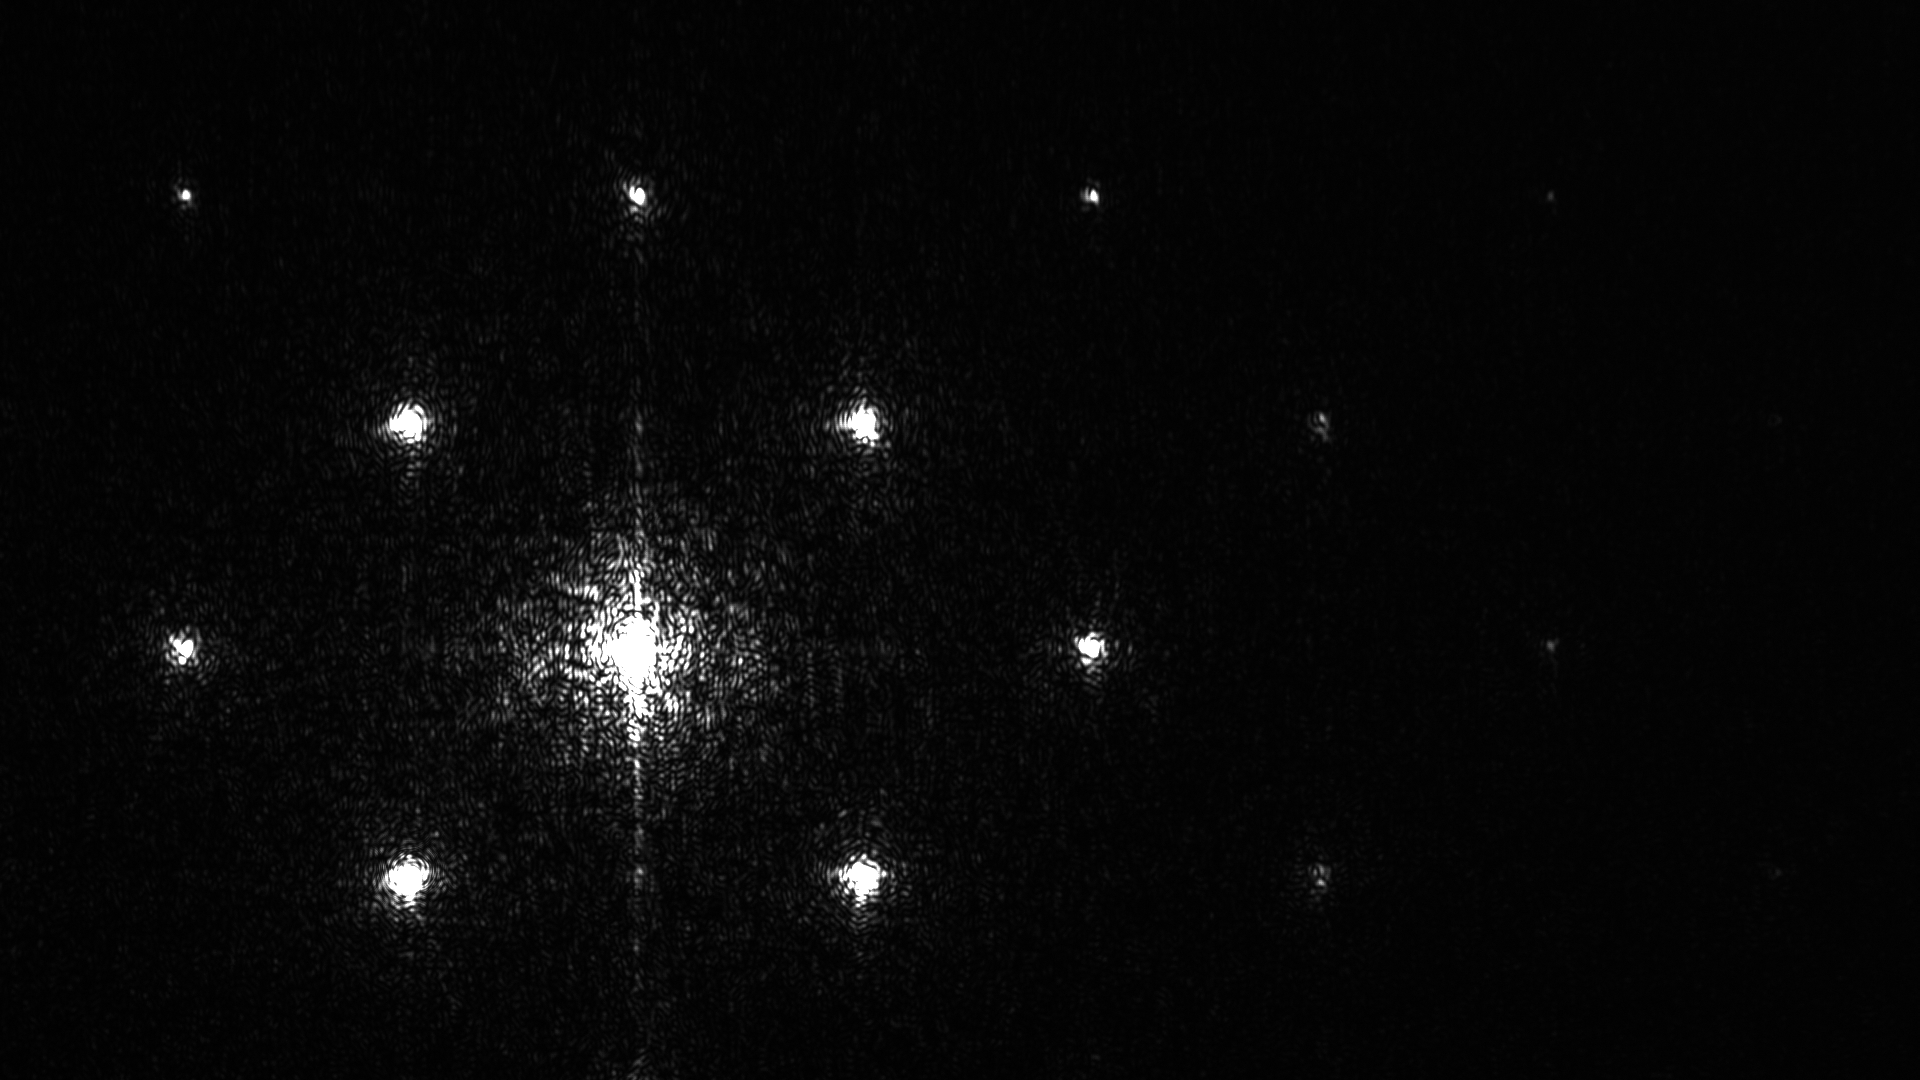
\includegraphics[scale=0.15]{/parte3-fourier/fourier-car-multiplied-pixels.png}
    \caption{Espectro de Fourier imagen autos }
    \label{fourier2}
    \end{figure}
    
    \begin{figure}[h]
    \centering
    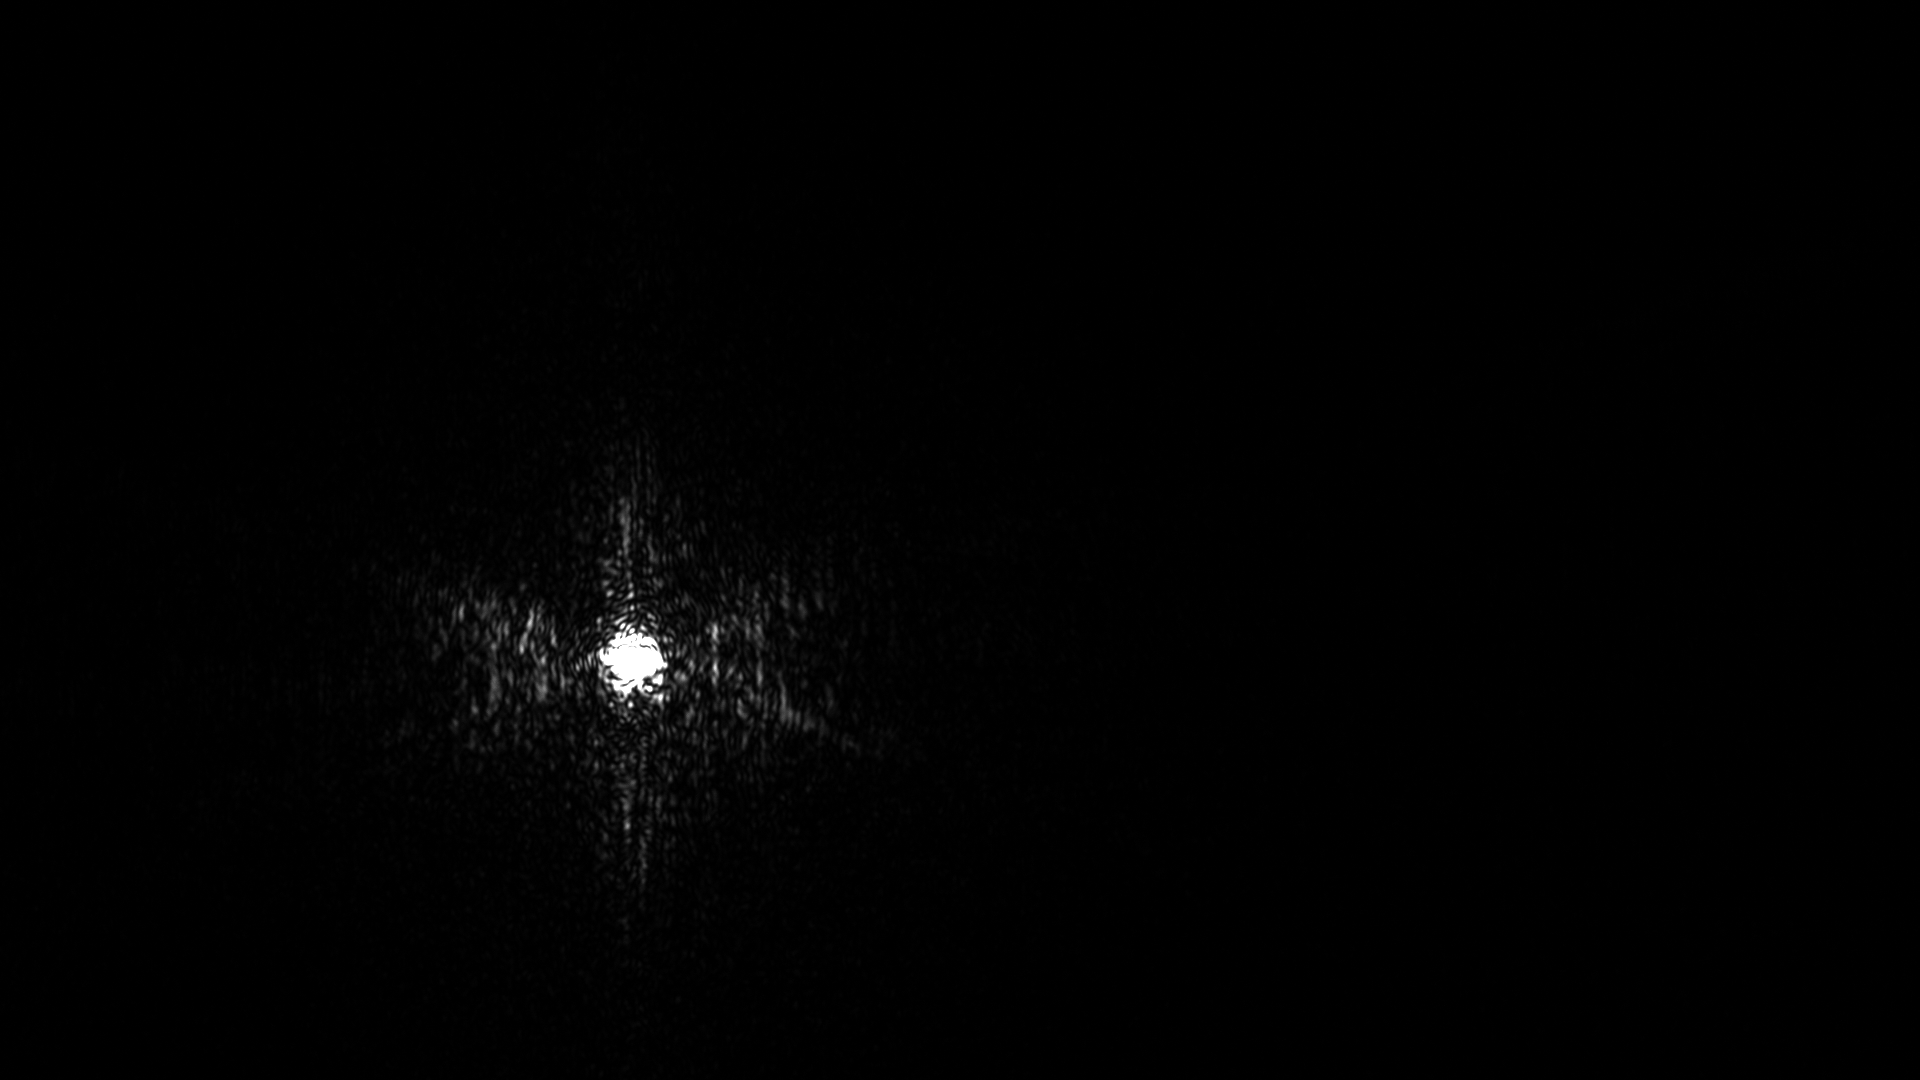
\includegraphics[scale=0.15]{/parte3-fourier/fourier-letras.png}
    \caption{Espectro de Fourier imagen letras. }
    \label{fourier3}
    \end{figure}
    
    \begin{figure}[h]
    \centering
    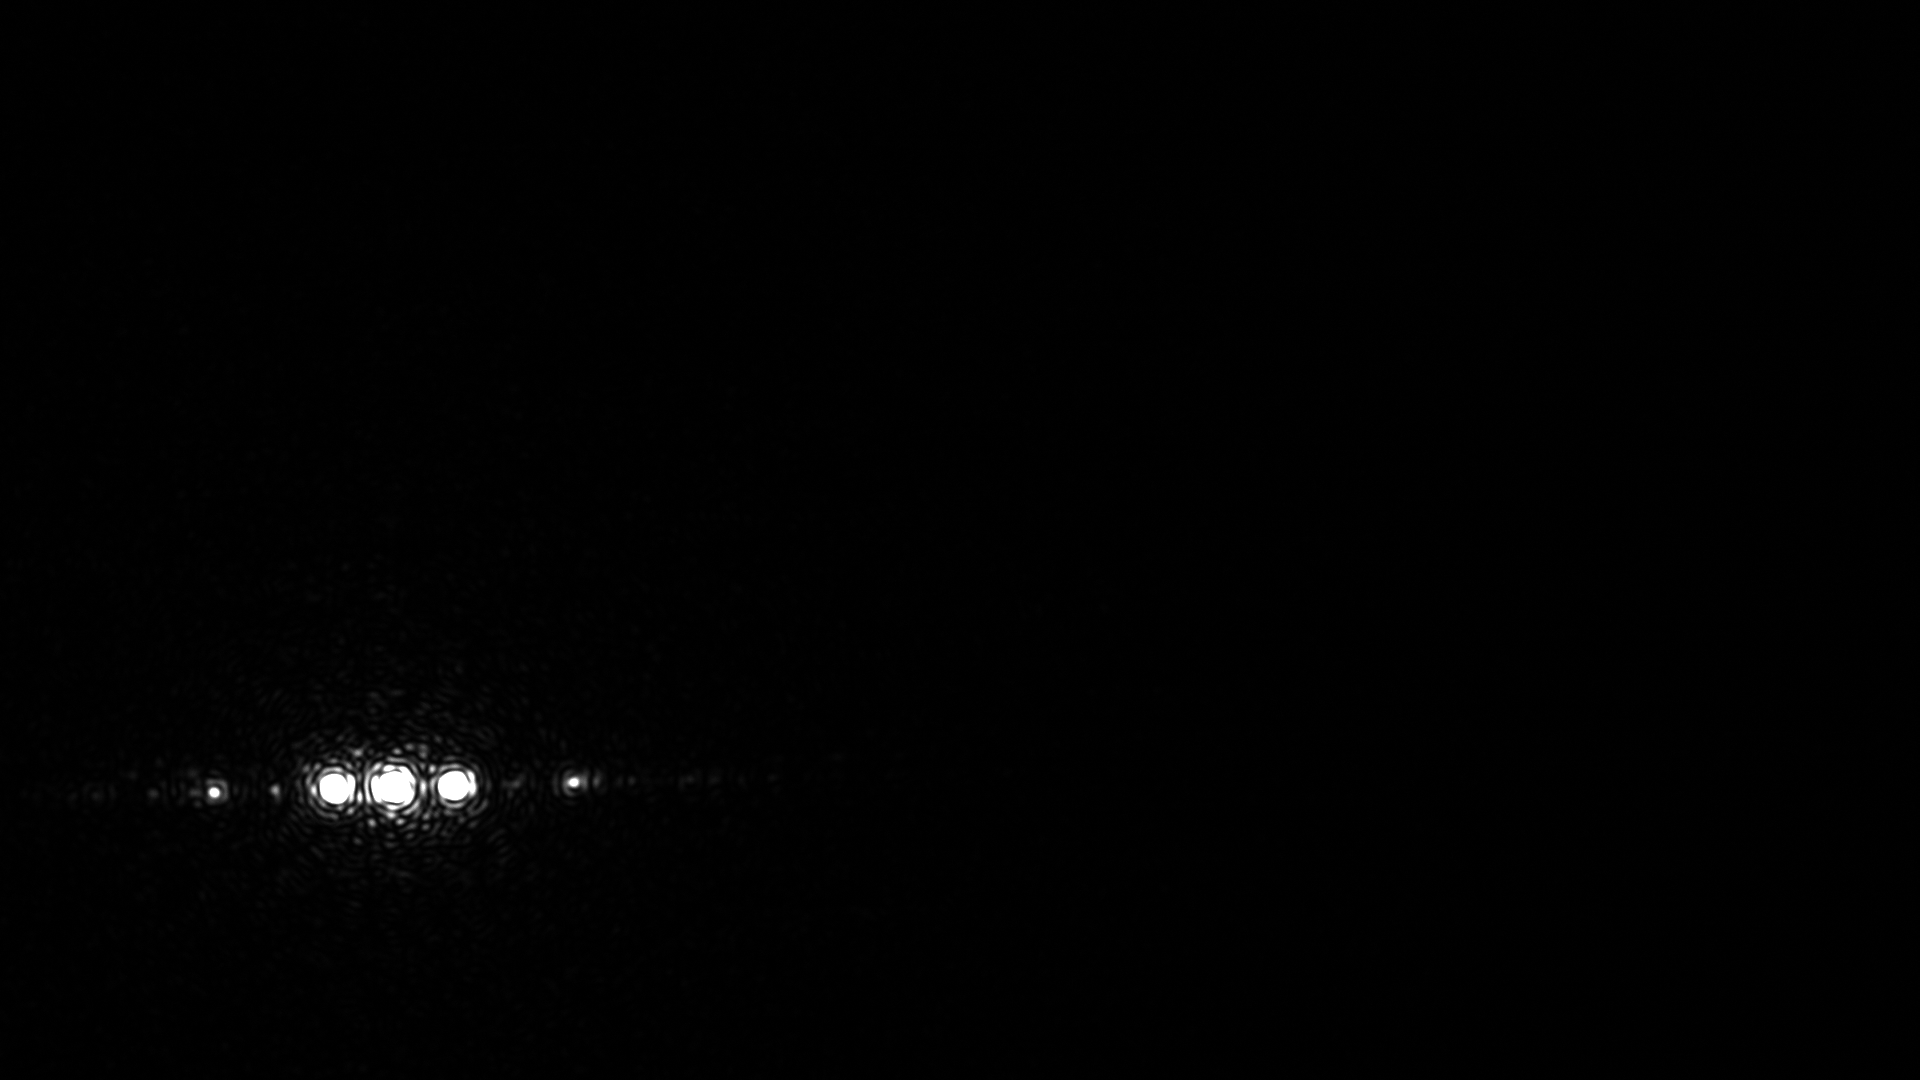
\includegraphics[scale=0.15]{/parte3-fourier/fourier-periodic-grating-10cm-focal.png}
    \caption{Espectro de Fourier imagen gratin }
    \label{fourier4}
    \end{figure}
    
A partir del espectro de Fourier estimar el periodo de la red aplicada para la observación del efecto del efecto de Talbot.


    \item Filtrado óptico
    \item Edad del Hierro
\end{enumerate}

\section{Resultados experimentales}

\subsection{Observación del efecto Talbot}

\subsubsection{Representando una señal óptica periódica (longitud de onda $\lambda$, periodo $d$) como una serie de Fourier, demostrar analíticamente que en las distancias iguales a la mitad de la distancia de Talbot, $z=\flatfrac{ZT}{2}$, observamos el objeto original desplazado en la mitad del periodo $d$.
}
\subsubsection{Usando las ecs. (7)-(8) analizar la intensidad y la fase del campo difractado por un objeto periódico compuesto de líneas blancas (transparentes) y negras (opacas) alternadas de la misma anchura, a una distancia $z=\flatfrac{ZT}{4}$}
\subsubsection[]{\begin{enumerate}
		\item Justifique el procedimiento seguido para determinar la distancia de Talbot y el periodo de la red y exponga los resultados.
		\item ¿Las imágenes observadas siempre son periódicos? ¿La respuesta está de acuerdo con la teoría?
	\end{enumerate}}


\subsection{Observación del espectro de Fourier}
\subsubsection{¿Qué valores d1 y d2 son adecuados para la observación del espectro de Fourier?}
\subsubsection[]{\begin{enumerate}
		\item ¿El espectro de la red está de acuerdo con la teoría (véanse los resultados del problema 1.6.)?
		\item Justifique el procedimiento seguido para determinar el periodo de la red y exponga los resultados.
	\end{enumerate}}
\subsubsection{¿Es posible registrar el espectro de Fourier colocando un objeto detrás de la lente?}



\subsection{Filtrado óptico}
\subsubsection{¿Qué distancia focal tiene la lente más próxima a la camera? Justifique el procedimiento seguido para determinar el orden de las lentes.}
\subsubsection{Elegir un filtro entre los estudiados en la práctica que podría ser adecuado para la observación de objetos semi-transparentes. Justifique la respuesta.}
\subsubsection{¿Qué observamos en la salida del sistema si usamos como filtro una red periódica? Justifique la respuesta.}

\subsection{Formación de imágenes con luz parcialmente coherente}

\subsubsection{¿El rango de distancias donde observamos la imagen del objeto 2D es mayor en el caso iluminación coherente o parcialmente coherente? ¿Qué iluminación es mejor para la observación de objetos 3D?}

\subsubsection{Para el sistema de filtrado usado en la práctica, la última lente es la pupila de salida del sistema. Determinar la respuesta impulsional y la función de transferencia del sistema en el caso de iluminación (a) coherente; (b) incoherente.}
%%%%%%%%%% If using BibTeX:
\bibliography{bibliography}

\end{document}
